% Minh họa lượng tử hóa, vẽ lại từ ảnh tham chiếu.
\begin{tikzpicture}[
    x=1.55cm,
    y=8.5cm,
    font=\small,
    line cap=round,
    line join=round
]
    \definecolor{quantizationsample}{RGB}{55, 153, 225}

    % Khung đồ thị và đường chuẩn tại mức 0.
    \draw[black!65, line width=0.45pt]
        (0, -0.335) rectangle (8.75, 0.395);
    \draw[black!55, line width=0.5pt] (0, 0) -- (8.75, 0);

    % Vạch chia thời gian, không ghi nhãn như trong ảnh.
    \foreach \position in {1,...,8} {
        \draw[black!65, line width=0.4pt]
            (\position, -0.335) -- (\position, -0.320);
        \draw[black!65, line width=0.4pt]
            (\position, 0.395) -- (\position, 0.380);
    }

    % Vạch chia và nhãn biên độ hai bên khung.
    \foreach \level/\labeltext in {
        -0.3/{-0.3}, -0.2/{-0.2}, -0.1/{-0.1},
        0/{0}, 0.1/{0.1}, 0.2/{0.2}, 0.3/{0.3}
    } {
        \draw[black!65, line width=0.4pt]
            (0, \level) -- (0.085, \level);
        \draw[black!65, line width=0.4pt]
            (8.75, \level) -- (8.665, \level);
        \node[anchor=east, text=black!70, inner sep=0pt]
            at (-0.09, \level) {$\labeltext$};
    }

    % Các mẫu và vòng tròn rỗng ở đầu mỗi vạch.
    % Giữ vị trí các đầu mẫu theo ảnh, kể cả mẫu mang nhãn 0.186.
    \foreach \position/\amplitude in {
        2/0.342, 4/0.3521, 6/0.156, 8/-0.1
    } {
        \draw[quantizationsample, line width=0.5pt]
            (\position, 0) -- (\position, \amplitude);
        \draw[quantizationsample, fill=white, line width=0.5pt]
            (\position, \amplitude) circle[radius=2.2pt];
    }

    % Nhãn biên độ và các nét chỉ vào đầu mẫu.
    \draw[->, >=stealth, line width=0.65pt]
        (4.25, 0.341) to[bend right=12] (4.05, 0.3521);
    \node[anchor=west, inner sep=0pt, font=\large\bfseries\boldmath]
        at (4.40, 0.330) {$0.3521\,\mathrm{V}$};

    \draw[->, >=stealth, line width=0.65pt]
        (6.25, 0.169) to[bend right=12] (6.06, 0.156);
    \node[anchor=west, inner sep=0pt, font=\large\bfseries\boldmath]
        at (6.30, 0.181) {$0.186\, \mathrm{V}$};

    \draw[->, >=stealth, line width=0.65pt]
        (8, -0.139) -- (8, -0.112);
    \node[anchor=north, inner sep=0pt, font=\large\bfseries\boldmath]
        at (8, -0.155) {$-0.1\,\mathrm{V}$};

    % Hai đường ngang minh họa giới hạn của một mức lượng tử.
    \node[anchor=east, inner sep=0pt, font=\large]
        at (3.34, 0.0625) {$\Delta_x=\dfrac{1}{8}$};
    \draw[line width=1.25pt] (3.50, 0.100) -- (3.90, 0.100);
    \draw[line width=1.25pt] (3.50, 0) -- (3.90, 0);

    % Hai mũi tên thẳng từ ngoài hướng vào hai đường giới hạn.
    \draw[->, >=stealth, line width=1.25pt]
        (3.70, 0.155) -- (3.70, 0.100);
    \draw[->, >=stealth, line width=1.25pt]
        (3.70, -0.055) -- (3.70, 0);
\end{tikzpicture}
